\chapter{Organisation}
\section{Metode}
En organisationsanalyse har til formål at belyse opbygningen af organisationen, hvori teknologien skal implementeres, i forhold til tilrettelæggelse og opgavefordeling. 
Det ønskes at undersøge de organisatoriske forudsætninger samt mulige (?) konsekvenser ved implementering af et (…)-aktivitetsarmbånd til monitorering i den primære sektor. Dette gøres ud fra et udgangspunkt i den modificerede Leavitt organisationsmodel samt samtaler med alment praktiserende læge (...?) for at analysere konsekvenserne af en eventuel ændring i organisationen. Leavitts modificerede organisationsmodel benyttes, da denne tager højde for omgivelsernes påvirkning på teknologi, aktører, opgaver, struktur, disses indbyrdes påvirkning og påvirkning på omgivelserne.

\begin{figure}[H]
\centering
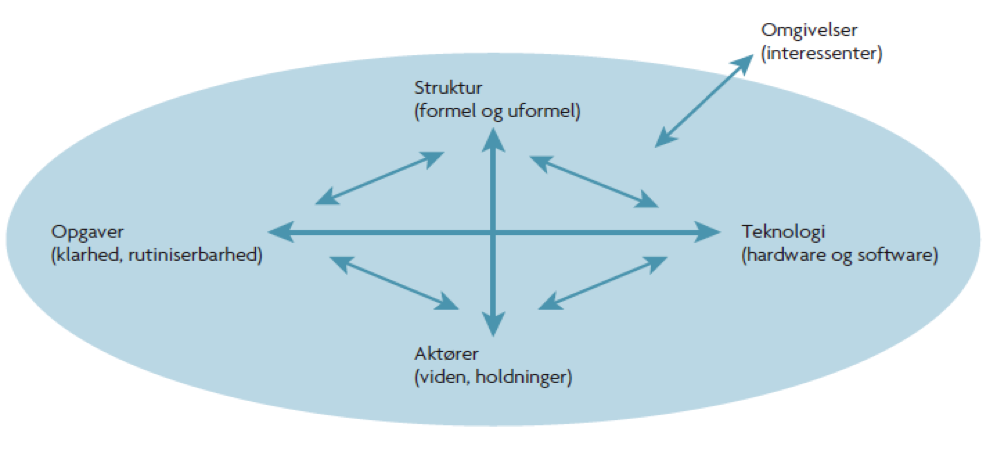
\includegraphics[width=0.9\textwidth]{figures/leavitt}
\caption{Leavitts modificerede organisationsmodel.}
\label{fig:leavittmodel}
\end{figure}

Dette giver anledning til følgende MTV-spørgsmål:

\subsection{MTV-spørgsmål}
\begin{itemize}
\item Hvordan passer  (…)-aktivitetsarmbånd ind i den nuværende organisation? 
\item Hvilke krav vil implementering af (…)-aktivitetsarmbånd stille til alment praktiserende læger, og hvem skal stå for en eventuel efteruddannelse? 
\begin{enumerate}
\item Hvor nemt/svært/tidskrævende er det at analyse data fra et sådant armbånd?
\item Hvornår er det ”nok” aktivitet til, at det kan bruges som et værktøj? Hvor går grænsen, og er det let at se om denne overskrides? 
\item Efteruddannelse/information/oplæg på konference, som kun nogle læger deltager i? Hvad vil dette betyde, hvis man har en ”gammeldags” læge?  Skal det være et tilbud fra alle læger, og hvordan sørger man for dette?
\end{enumerate}
\item  Hvordan vil arbejdsfordelingen mellem den primære og sekundære sundhedssektor blive påvirket, og hvad vil en ændring i arbejdsfordelingen medføre?
\begin{enumerate}
\item Hvor mange patienter bliver på nuværende tidspunkt henvist til sekundære sundhedssektor
\end{enumerate} 
\end{itemize}